\documentclass[conference]{IEEEtran}
\IEEEoverridecommandlockouts
% The preceding line is only needed to identify funding in the first footnote. If that is unneeded, please comment it out.
\usepackage{cite}
\usepackage{amsmath,amssymb,amsfonts}
\usepackage{algorithmic}
\usepackage{graphicx}
\usepackage{textcomp}
\usepackage{xcolor}
\usepackage{array}
%\usepackage{adjustbox}
\def\BibTeX{{\rm B\kern-.05em{\sc i\kern-.025em b}\kern-.08em
    T\kern-.1667em\lower.7ex\hbox{E}\kern-.125emX}}
\begin{document}

\title{Explainable Artificial Intelligence \\ {Methodology for Handwritten Applications}}

\author{\IEEEauthorblockN{Paul Whitten, Francis Wolff, Chris Papachristou}
\IEEEauthorblockA{\textit{Electrical, Computer, and Systems Engineering} \\
\textit{Case School of Engineering} \\
\textit{Case Western Reserve University} \\
Cleveland, OH, USA \\
pcw@case.edu, fxw12@case.edu, cap2@case.edu}

}

\maketitle

\begin{abstract}
There has been explosive growth of practical AI in recent years.
%However, inferential results of AI systems are not readily explainable to humans.
A major concern of current AI systems and compliance regulations is an inability to explain inferential decisions.
%Explainable artificial intelligence has been posed to mitigate these concerns.
This work explores an Explainable Artificial Intelligence (XAI) methodology that provides explanations
for classification decisions.  Experimental results using the MNIST handwritten digit database are provided with explainable conclusions.
\end{abstract}

\begin{IEEEkeywords}
explainable, artificial intelligence, machine learning, AI regulations
\end{IEEEkeywords}

\section{Introduction}

Recent advances in Machine Learning (ML) have brought about wide adoption of ML
algorithms for many applications.  Despite various successes, there is a
reluctance to adopt ML in some applications because ML behaves like an opaque
box where the internal structures are not understood.  Thus, this type of
decision-making is not explainable or useful to humans. 

The EU law related to the General Data Protection Regulation\cite{gdpr2016},
indicates a controller shall provide a data subject with meaningful information
about the logic involved in automated decision making or profiling.  Other
countries are considering AI legislation, especially the US\cite{burt_2021}.
There is debate over the right to an explanation when using AI in significant
decisions\cite{selbst}.  The motivation for this work is the need for
explainability in AI.

%\begin{figure}[htbp]
%\centerline{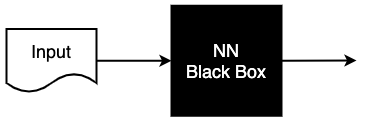
\includegraphics[width=40mm]{./images/unexplainable.png}}
%\caption{An unexplainable NN.}
%\label{unexplainable}
%\end{figure}

%\begin{figure}[htbp]
%\centerline{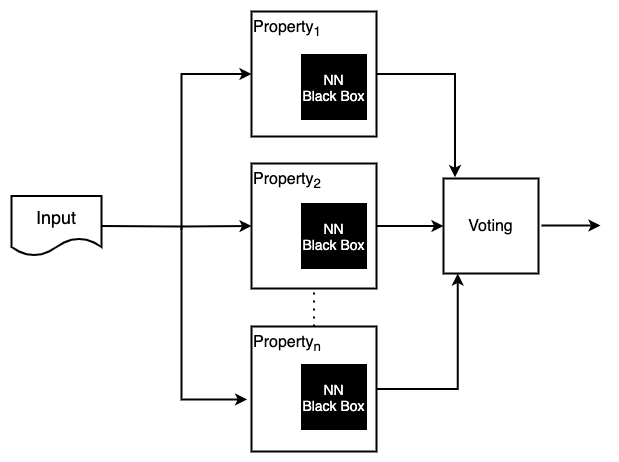
\includegraphics[width=95mm]{./images/explainable.png}}
%\caption{Fine grained explainable NN classification based on properties.}
%\label{explainable}
%\end{figure}

This work approaches the widely studied problem of classifying images of
handwritten digits into the ten decimal digit classes from an XAI perspective.
The goal is to provide explainable classification in the form of rationale that
a layperson can understand.  This is achieved using an explainable architecture,
with fine-grained classification decisions based on explainable properties, and
a methodology for constructing the explainable architecture.  This work does not
attempt to explain the internal structure of the ML model.  In this work, ML
models still act as opaque entities, but through finer-grained classification,
an element of explainability is added.

Herein, the methodology and architecture are applied, using the MNIST
handwritten digit database \cite{deng2012mnist}.  Next, the approach is outlined
along with test cases and examples of explainability.  Finally, results and
metrics to gauge accuracy and explainability are presented.

This work poses a means of explaining classification to a human.  The intent is
not to compete with established algorithms that perform exceptionally well in
classification of input \cite{keysers07} \cite{lecun98} \cite{schm2012}.  The
effort required to apply the methodology is significant compared to training a
classifier that is not explainable.

While XAI is approached for a specific classification problem, in the MNIST
handwritten digit database, the methodology translates to other challenges
requiring explainable classification among a finite set of classes.

\section{Related work}

The ability to map the learning classifier or recognizer to human-based
explainability is a challenging task for human understandability.  Currently,
there are at least seventeen explainable techniques such as decision tree-based,
rule-based (i.e. knowledgebase), salience mapping, sensitivity-based analysis,
feature importance, fuzzy-based, neural-network, and genetic-programming based.
These techniques use one of three basic evaluation approaches:
application-grounded, human-grounded and functionally grounded
\cite{Arrieta2020ExplainableAI,Survey18,Fuzzy19,Hagras18,GP18}.

Distributed and fault tolerant systems research has provided several examples of
voting \cite{avizienis} and probabilistic models for the voting problem
\cite{blough}.

\begin{figure}[htbp]
\centerline{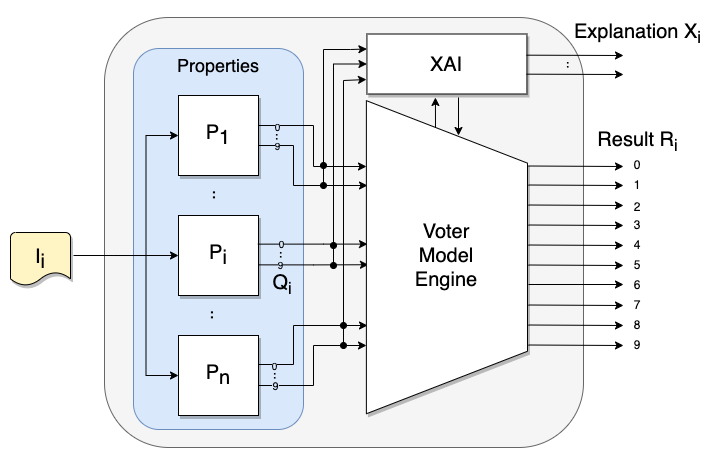
\includegraphics[width=90mm]{./images/voting_prop_nn_2.png}}
\caption{XAI Architecture}
\label{voting}
\end{figure}

\section{Overview}


Explainable properties and related input transformations are the basis for the
explainable methodology.  The architecture performs distinct classification
decisions for each property transformation.  Those distinct classifications are
input to a voter to provide a final classification decision.  Explainability
comes from relating the fine-grained decisions, for property transformations, to
compose rationale for a user.

Fig.~\ref{voting} depicts the explainable architecture.  $I_i$ represents the
$i$th input to the architecture.  The architecture consists of Properties, a
Voter Model Engine (VME),  and an Explainable Artificial Intelligence block.
Explainable properties are defined as descriptive qualities of a sample input
that mean something to a user in the problem domain, especially to justify a
classification decision.   Explainable properties $P_1$ through $P_n$ are
outlined in the blue Properties rectangle.  Each property represents logic for a
classification based solely on the property.   $Q_j$ represents the $j$th
property's classification output.

The VME relies on classifications from the explainable properties, $Q_j$, and
feedback from the XAI block to make a final classification decision.   Two
voting schemes are discussed in the approach section.

The XAI block, in Fig.~\ref{voting}, consists of a knowledgebase and logic to
generate an explanation for the user.  Inputs to the XAI block are explainable
property classifications and the VME decision.  The XAI knowledgebase contains
information on explainable properties, training results, and metrics related to
the effectiveness of properties.  The explanation provided by the XAI block
consists of rationale that relates to the explainable properties contributing to
the classification decision.

 \begin{figure}[htbp]
\centerline{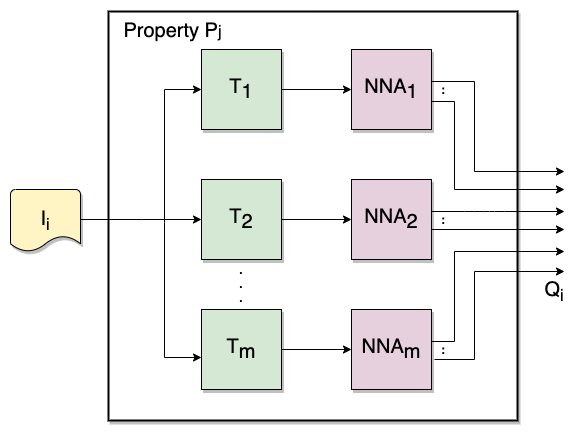
\includegraphics[width=90mm]{./images/property_transforms.png}}
\caption{Architecture of a single property for multiple transformations.}
\label{proptrans}
\end{figure} 

A property transformation is a modifying function applied to the input.
Transformations identify the explainable property in the input.  Each property
may have one or more transformations.   Fig.~\ref{proptrans} represents
transformations in the explainable architecture.  The outer square represents
the $j$th property from Fig.~\ref{voting}.  The boxes labeled $T_1$ through
$T_m$ indicate $m$ transformations of the input related to property $j$.
Transformed input is fed to a trained Neural Network Architecture (NNA) to make
classification decisions.  Classification output then flows to the VME as shown
in Fig.~\ref{voting}.

\section{Methodology}
 
Our methodology for achieving explainable ML classification involves the
following steps:
%\begin{itemize}
%\item Discover explainable properties.
%\item Define transformations for explainable properties.
%\item Transform training data.
%\item Produce trained explainable property-specific NNAs.
%\item Build a Knowledgebase across the explainable properties.
%\item Devise a voting scheme.
%\item Use a test dataset to provide feedback.
%\end{itemize}

\subsubsection{Discover Explainable Properties}
An explainable property is an attribute of a sample in the problem domain that
may differentiate classes and provide a rationale for a classification decision
to a user.   An explainable property need not be present in all classes.
Discovering explainable properties may require manual analysis of sample inputs.

\subsubsection{Define and Implement Transformations}
Data transformations are next defined and implemented to highlight explainable
properties in the input.  Transforms may be known algorithms of feature
detection and extraction that relate to explainable properties.

\subsubsection{Transform Training Data} 
A transformed training dataset is generated by submitting all elements from the
training set to the property transformations.  The output from property
transformations is stored for later use in training the property transform
specific NNAs. 

\subsubsection{Produce Trained Property NNAs}
The next step involves initializing unique NNAs for each property
transformation.  The NNAs are trained, using supervised ML techniques, from the
data stored in the previous step.  The result is a set of trained NNAs that
produce classifications for the explainable property transforms.

\subsubsection{Build an XAI Knowledgebase}
After training the NNAs, the training set is processed again to populate the XAI
knowledgebase with the property classification results.  The knowledgebase also
stores explainable property descriptions and each property's classification
result for the training data.  Metrics on the per-class effectiveness of
explainable properties are calculated and stored in the knowledgebase.

\subsubsection{Devise a Voting Scheme}
The purpose of the voting scheme is to decide among the potentially conflicting
votes from the explainable property transformation classifications.  Information
from the knowledgebase and explainable property classifications are input to the
voting scheme.  Probabilistic and ML based voting schemes are discussed in the
approach section.

\subsubsection{Provide User Feedback}
Finally, when test data are presented to the architecture, the results are
evaluated to determine if they are sufficient.  The performance of the
explainable property transforms are examined for effectiveness.  Classes with
poor results are identified and new properties or transforms are sought where
there are gaps.

\section{Approach}

This section presents the approach of applying the methodology to the MNIST
handwritten digit database. 

\subsection{Explainable Properties}

Through a manual review of samples in MNIST, explainable properties related to
shapes and characteristics of the digits are identified.  The explainable
properties utilized are listed in the Property column of
Table~\ref{transsample}.

\subsection{Transformations}
 
Digital image processing techniques that highlight the explainable properties
are used as transforms.  The Transform column in Table~\ref{transsample} lists
transformations for the various properties.  The figure also shows example MNIST
digits, $I_i$, and their resulting transformed images, $T_j(I_i)$.

\bgroup
\renewcommand{\arraystretch}{1.8}
%\setlength\tabcolsep{2mm}
\begin{table}
\renewcommand{\arraystretch}{1.3}
\caption{Properties and transforms for the MNIST example}
\centering
\resizebox{\columnwidth}{!}{%
\begin{tabular}{ c | p{0.23\linewidth} | p{0.23\linewidth} | ccc | }
\cline{2-6}
$P_j$ & Property & Transform & $I_i$ &  &  $T_j(I_i)$ \\
\hline \hline
$P_1$ & Stroke & Skeleton & \raisebox{-.5\height}{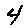
\includegraphics[width=5.5mm]{./digit-images/4-11.png}} & $\rightarrow$ & \raisebox{-.5\height}{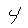
\includegraphics[width=5.5mm]{./digit-images/4-11-skel.png}} \\
\hline
$P_2$ & Circle & Hough Circle & \raisebox{-.5\height}{
\includegraphics[width=5.5mm]{./digit-images/6-17.png}} & $\rightarrow$ & \raisebox{-.5\height}{
\includegraphics[width=5.5mm]{./digit-images/6-17-circle.png}} \\
\hline
$P_3$ & Crossings & Crossings & \raisebox{-.5\height}{
\includegraphics[width=5.5mm]{./digit-images/4-2.png}} & $\rightarrow$ & \raisebox{-.5\height}{
\includegraphics[width=5.5mm]{./digit-images/4-2-crossing.png}} \\
\hline
$P_4$ & Circle & Hough Ellipse & \raisebox{-.5\height}{
\includegraphics[width=5.5mm]{./digit-images/0-3.png}} & $\rightarrow$ & \raisebox{-.5\height}{
\includegraphics[width=5.5mm]{./digit-images/0-3-ellipse.png}} \\
\hline
$P_5$ & Circle & Multiple Ellipse Circle & \raisebox{-.5\height}{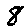
\includegraphics[width=5.5mm]{./digit-images/8-4.png}} & $\rightarrow$ & \raisebox{-.5\height}{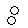
\includegraphics[width=5.5mm]{./digit-images/8-4-ellipse-circle.png}} \\
\hline
$P_6$ & Endpoints & Endpoints & \raisebox{-.5\height}{
\includegraphics[width=5.5mm]{./digit-images/2-2.png}} & $\rightarrow$ & \raisebox{-.5\height}{
\includegraphics[width=5.5mm]{./digit-images/2-2-endpoint.png}} \\
\hline
$P_7$ & Enclosed Region & Flood Fill & \raisebox{-.5\height}{
\includegraphics[width=5.5mm]{./digit-images/0-2.png}} & $\rightarrow$ & \raisebox{-.5\height}{
\includegraphics[width=5.5mm]{./digit-images/0-2-fill.png}} \\
\hline
$P_8$ & Line & Hough Line & \raisebox{-.5\height}{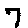
\includegraphics[width=5.5mm]{./digit-images/7-20.png}} & $\rightarrow$ & \raisebox{-.5\height}{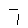
\includegraphics[width=5.5mm]{./digit-images/7-20-line.png}} \\
\hline
$P_9$ & Enclosed Region & Skeleton Flood Fill & \raisebox{-.5\height}{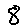
\includegraphics[width=5.5mm]{./digit-images/8-3.png}} & $\rightarrow$ & \raisebox{-.5\height}{
\includegraphics[width=5.5mm]{./digit-images/8-3-skel-fill.png}} \\
\hline
\end{tabular}%
}
\centering
\label{transsample}
\end{table}
\egroup

The Stroke property, $P_1$, is meant to represent the minimal path of the
writing implement to trace the digit.  The morphological skeleton transformation
is a one-pixel connected representation of the digit,  representing the stroke.
The Lee\cite{Lee1994} algorithm for the skeleton is used. $P_2$, $P_4$, and
$P_5$ are the circle property with corresponding transforms $T_2$, $T_4$, and
$T_5$ representing the Hough Circle, the Hough Ellipse, and multiple
non-overlapping circles and ellipses. $P_3$ and $T_3$ are the crossings property
and transform representing the intersection of line segments in a digit.  $T_3$
involves taking the skeleton and then finding activated pixels with more than
two neighbors.   The endpoints property and transform, $P_6$ and $T_6$, involved
taking activated pixels in the skeleton with only one neighbor. Property $P_7$
and $P_9$ for enclosed regions used transform $T_7$ which involved a flood fill
and $T_9$ the flood fill of the skeleton.  The line property and transform,
$P_8$ and $T_8$, uses an algorithm to find the non-overlapping Hough Lines.

\subsection{Transforming Training Data}

The various transforms are applied to MNIST images using implementations in the
Python scikit-image library \cite{scikitimage}.  The resulting transformed
images are stored for each property transform to be used for training NNAs.

\subsection{Training}

The trained NNAs are implemented using Python scikit-learn Multi-Layer
Perceptrons \cite{scikitlearn}.  The property transform NNAs are trained using
the transformed data stored in the previous step.

\subsection{Knowledgebase}

After training the NNAs, the transformed training data are presented to the NNAs
and results are stored.  Data are later loaded to in-memory maps,  for efficient
runtime access, while performing metric calculation.  Textual property labels
and descriptions are also stored in the knowledgebase for composing explainable
rationale in the XAI block.

\subsection{Voting Schemes}
\label{subsection:Voting}

The first voting scheme is probabilistic.  In this scheme, the knowledgebase is
used to identify each explainable property transformation's effectiveness to
correctly predict a digit.   The effectiveness for an explainable property
transformation, $j$, to select a particular digit, $d$,  is given by:
\begin{equation}\label{effectiveness}
E_{j,d}  = \frac{|A|}{|B|}
\end{equation}
where $A$ is the set of correct classifications of explainable property
transformation $j$ of the digit $d$ and $B$ is the set of elements of digit $d$.
The weight of the effectiveness for each digit, $d$, is:
\begin{equation}\label{weight}
W_d=\sum_j E_{j, d}
\end{equation}
The confidence for the digit $d$ is calculated by the VME and is given by:
\begin{equation}\label{conf}
C_d=\frac{W_d}{\sum\limits_kW_k}
\end{equation}
The denominator is the sum of all weights for classes selected by a property.
If multiple digits are selected by the properties, the digit with the highest
confidence will be chosen by the VME.

The second voting scheme is NN based.  Explainable property transformation
output and labels, from the knowledgebase, are used to train a Multi-Layer
Perceptron model in the NN VME.

\subsection{ User Feedback}

Hough circles are effective for detecting digits six and nine but perform poorly
for digits eight and zero.  The ellipse is better in extracting characteristics
of handwritten zeros.   A transform that used multiple non-overlapping circles
or ellipses improved detection for the digit eight.  As implemented, the
inflection point property and corner detection transforms gave poor results for
all digit classes, so the property was eliminated.

\section{Examples}

Detailed examples from MNIST follow in this section by first providing aggregate
property classification results for the digits five and six and then explainable
results from three different input images.

Tables ~\ref{table:digit5out} and ~\ref{table:digit6out} show the property
transformation NNA output and statistics, stored in the knowledgebase, for
digits five and six.  Columns labeled $P_1$ through $P_9$ of the tables
represent the property transformations, $P_j$, from Table~\ref{transsample}.
The first row of the tables represents effectiveness, $E_{j,d}$, where $j$ is
the property transform, and $d$ is the digit.  An example of effectiveness can
be observed for $E_{2,5}=0.14$ in row 1 column 2 of Table \ref{table:digit5out}.
where $P_2$, Hough Circle, only got $\frac{772}{5421}=0.14$ fives correct.   The
second, third, and fourth rows represent the standard deviation, kurtosis, and
skew of the digit outputs for each property.  The numbered rows in the tables
represent the means of the property outputs for each digit.  The last two rows
are the false-positive and false-negative rates.

Observe that the Stroke property, $P_1$, performs very well in both digits.  The
next highest performing property in both tables is the endpoint property, $P_6$,
with 0.85 and 0.93 effectiveness.  The digit six also has good classification
results for the enclosed region properties, $P_7$ and $P_9$.  The digit six also
performs better than the five in the properties related to the circle, $P_2$,
$P_4$, and $P_5$.  The digit five has among the poorest performance as observed
from the relatively low percent correct and high false-negative rates.

\begin{table}
\renewcommand{\arraystretch}{1.3}
\begin{minipage}{0.48\textwidth}
\caption{Digit 5 Outputs}
%\centering
\resizebox{\columnwidth}{!}{%
%\begin{adjustbox}{width=\columnwidth,center}
\begin{tabular}{ | c ||  c | c | c | c | c | c | c | c | c |}
Digit 5 & $P_1$ & $P_2$ & $P_3$ & $P_4$ & $P_5$ & $P_6$ & $P_7$ & $P_8$ & $P_9$ \\
\hline \hline
$E_{j,5}$  & 1.00 & \textbf{0.14} & 0.57 & 0.21 & 0.22 & \textbf{0.85} & 0.04 & 0.70 & 0.06 \\
\hline
$\sigma$ & 0.30& 0.08& 0.08& 0.07& 0.09& 0.25& 0.07& 0.21& 0.08 \\
\hline
k & 10.0& 4.00& -1.86& 5.56& 6.23& 9.55& -1.94& 9.78& -2.06 \\
\hline
skew & 3.16& 1.91& 0.33& 2.32& 2.41& 3.07& -0.03& 3.12& 0.06 \\
\hline
0 & 0.00 & 0.12 & 0.21 & 0.09 & 0.07 & 0.00 & 0.01 & 0.02 & 0.02 \\
\hline
1 & 0.00 & 0.05 & 0.22 & 0.06 & 0.04 & 0.11 & 0.19 & 0.01 & 0.18 \\
\hline
2 & 0.00 & 0.05 & 0.05 & 0.06 & 0.05 & 0.00 & 0.09 & 0.03 & 0.07 \\
\hline
3 & 0.00 & 0.16 & 0.08 & 0.15 & 0.15 & 0.00 & 0.15 & 0.08 & 0.18 \\
\hline
4 & 0.00 & 0.05 & 0.01 & 0.06 & 0.05 & 0.00 & 0.12 & 0.02 & 0.13 \\
\hline
5 & 1.00 & 0.30 & 0.20 & 0.28 & 0.35 & 0.85 & 0.19 & 0.73 & 0.19 \\
\hline
6 & 0.00 & 0.10 & 0.07 & 0.06 & 0.09 & 0.01 & 0.03 & 0.04 & 0.04 \\
\hline
7 & 0.00 & 0.05 & 0.17 & 0.07 & 0.04 & 0.00 & 0.19 & 0.01 & 0.21 \\
\hline
8 & 0.00 & 0.11 & 0.02 & 0.09 & 0.10 & 0.01 & 0.01 & 0.04 & 0.01 \\
\hline
9 & 0.00 & 0.04 & 0.02 & 0.07 & 0.04 & 0.01 & 0.03 & 0.03 & 0.03 \\
\hline
false pos. \%  & 0.0 & 0.5 & 0.2 & 0.4 & 0.7 & 0.4 & 0.0 & 0.3 & 0.0 \\
\hline
false neg. \%  & 0.0 & 84.8 & 94.1 & 78.8 & 78.3 & 13.4 & 96.2 & 29.2 & 94.5 \\
\hline
\end{tabular}%
%\end{adjustbox}
}
\label{table:digit5out}
%\end{table}
\end{minipage}

%\begin{table}
\begin{minipage}{0.48\textwidth}
\caption{Digit 6 Outputs}
%\centering
\resizebox{\columnwidth}{!}{%
%\begin{adjustbox}{width=\columnwidth,center}
\begin{tabular}{ | c ||  c | c | c | c | c | c | c | c | c |}
Digit 6 & $P_1$ & $P_2$ & $P_3$ & $P_4$ & $P_5$ & $P_6$ & $P_7$ & $P_8$ & $P_9$ \\
\hline \hline
$E_{i,6}$  & 1.00 & 0.47 & 0.50 & 0.32 & 0.49 & \textbf{0.93} & 0.82 & 0.71 & 0.83 \\
\hline
$\sigma$ & 0.30& 0.11& 0.13& 0.09& 0.13& 0.26& 0.24& 0.21& 0.25 \\
\hline
k & 10.0& 8.51& 8.62& 9.86& 9.47& 9.96& 9.94& 9.89& 9.93 \\
\hline
skew & 3.16& 2.84& 2.89& 3.13& 3.05& 3.15& 3.15& 3.14& 3.15 \\
\hline
0 & 0.00 & 0.10 & 0.04 & 0.07 & 0.08 & 0.02 & 0.00 & 0.03 & 0.00 \\
\hline
1 & 0.00 & 0.05 & 0.05 & 0.07 & 0.05 & 0.01 & 0.04 & 0.01 & 0.03 \\
\hline
2 & 0.00 & 0.06 & 0.14 & 0.06 & 0.06 & 0.02 & 0.02 & 0.03 & 0.01 \\
\hline
3 & 0.00 & 0.10 & 0.05 & 0.07 & 0.08 & 0.00 & 0.03 & 0.05 & 0.03 \\
\hline
4 & 0.00 & 0.03 & 0.04 & 0.07 & 0.04 & 0.00 & 0.03 & 0.05 & 0.02 \\
\hline
5 & 0.00 & 0.10 & 0.07 & 0.05 & 0.09 & 0.01 & 0.03 & 0.03 & 0.02 \\
\hline
6 & 1.00 & 0.43 & 0.49 & 0.38 & 0.50 & 0.89 & 0.82 & 0.73 & 0.84 \\
\hline
7 & 0.00 & 0.06 & 0.05 & 0.08 & 0.05 & 0.00 & 0.03 & 0.01 & 0.04 \\
\hline
8 & 0.00 & 0.03 & 0.09 & 0.07 & 0.03 & 0.03 & 0.00 & 0.04 & 0.00 \\
\hline
9 & 0.00 & 0.03 & 0.03 & 0.08 & 0.04 & 0.00 & 0.01 & 0.03 & 0.01 \\
\hline
false pos. \%  & 0.0 & 2.6 & 2.5 & 0.5 & 2.2 & 0.7 & 0.2 & 0.6 & 0.0 \\
\hline
false neg. \%  & 0.0 & 53.3 & 50.1 & 67.5 & 50.7 & 6.6 & 18.1 & 28.1 & 16.8 \\
\hline
\end{tabular}%
%\end{adjustbox}
}
\label{table:digit6out}
\end{minipage}
\end{table}

Mean digit values from the Property NNAs are also represented  in
Fig.~\ref{digit5votes} and ~\ref{digit6votes} as three dimensional surface plots
for digits five and  and six.

\begin{figure}[htbp]
\begin{minipage}{0.48\textwidth}
\centerline{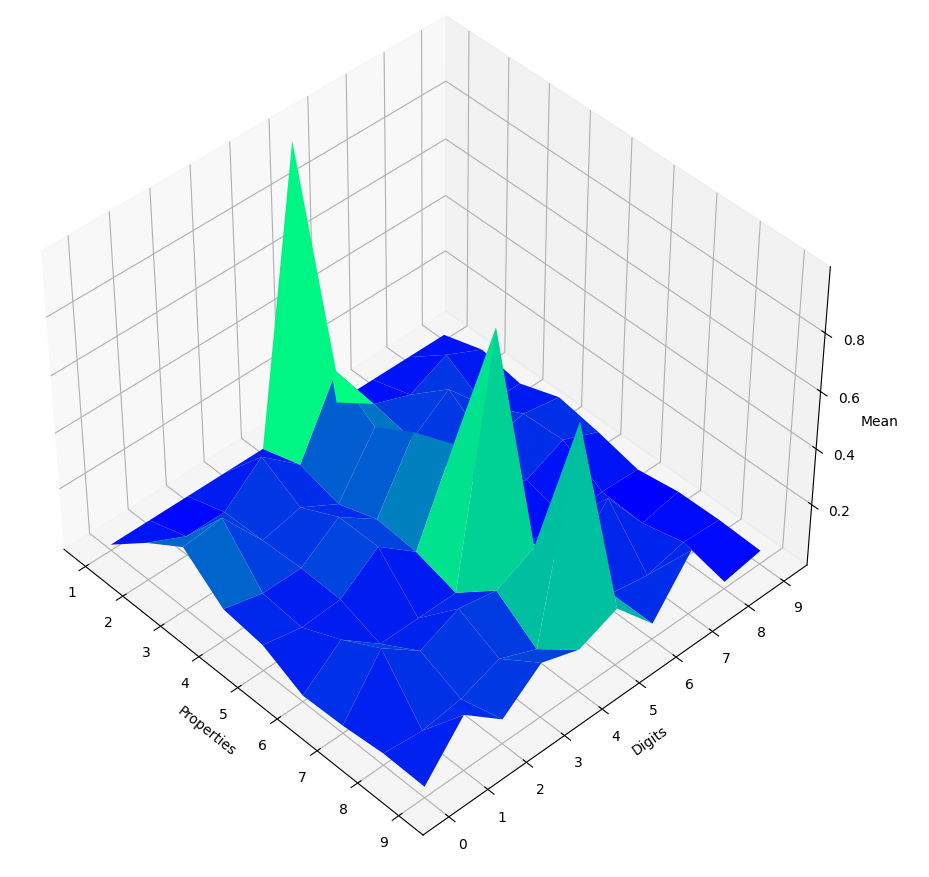
\includegraphics[width=70mm]{./images/digit-5.png}}
\caption{Property output for digit 5}
\label{digit5votes}
\end{minipage}
\begin{minipage}{0.48\textwidth}
\centerline{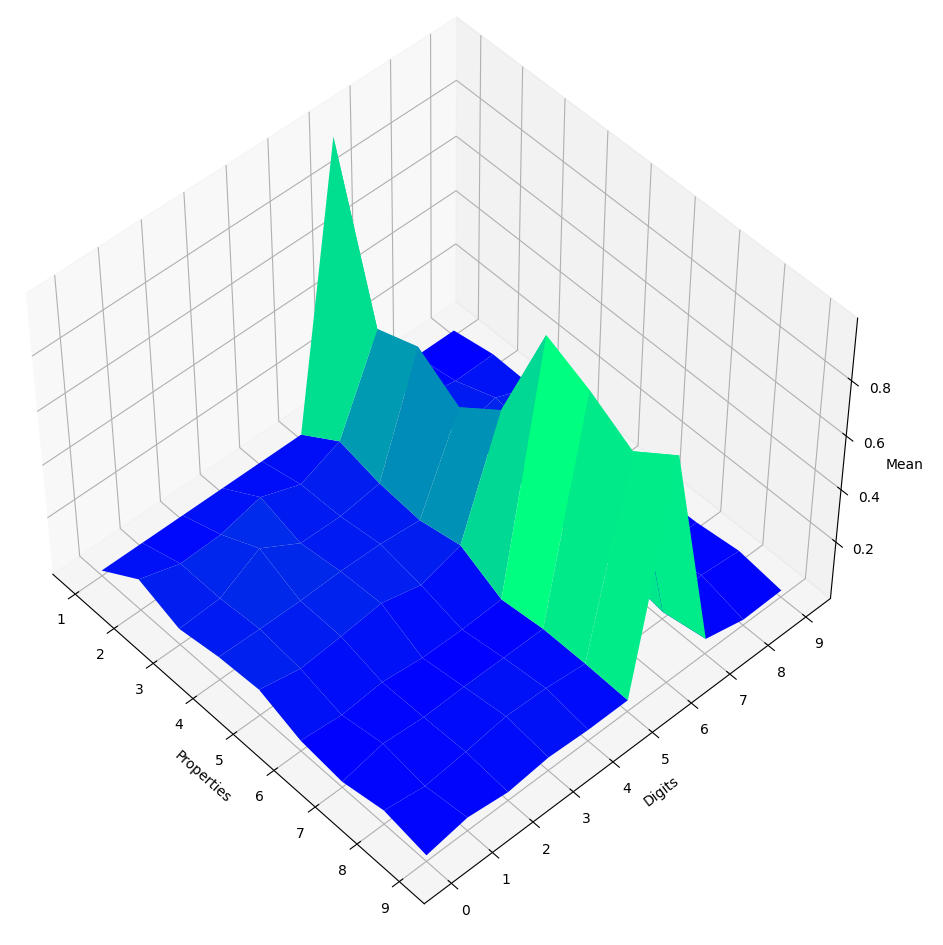
\includegraphics[width=70mm]{./images/digit-6.png}}
\caption{Property output for digit 6}
\label{digit6votes}
\end{minipage}
\end{figure}

%\begin{table}[htbp]
%\caption{Properties, Transforms and Property Identifiers}
%\centering
%\begin{tabular}{| c | c | c |}
%\hline
% Identifier & Explainable Property & Transform \\
%\hline\hline
%$P_1$ & Stroke & Skeleton \\
%\hline
%$P_x$ & Circle & Hough Circle \\
%\hline
%$P_x$ & Crossings & Crossing Point \\
%\hline
%$P_x$ & Ellipse & Hough Ellipse \\
%\hline
%$P_x$ & Ellipse + Circle & Hough Ellipse and Circle \\
%\hline
%$P_x$ & Endpoints & Endpoints \\
%\hline
%$P_x$ & Enclosed Region & Flood Fill \\
%\hline
%$P_x$ & Line & Hough Line \\
%\hline
%$P_x$ & Enclosed Region of Skeleton & Skeleton Flood Fill \\
%\hline
%\end{tabular}
%\label{table:tblproptrans}
%\end{table}

%\begin{figure}[htbp]
%\centerline{
\includegraphics[width=15mm]{./digit-images/5-0.png}}
%\caption{Example 1 of a handwritten digit five}
%\label{example1}
%\end{figure}

\begin{figure}[htbp]
\begin{minipage}{0.15\textwidth}
\centerline{
\includegraphics[width=15mm]{./digit-images/5-0.png}}
\caption{Example 1}
\label{example1}
\end{minipage}
 \begin{minipage}{0.15\textwidth}
\centerline{
\includegraphics[width=15mm]{./digit-images/9-9.png}}
\caption{Example 2}
\label{example2}
\end{minipage}
\begin{minipage}{0.15\textwidth}
 \centerline{
\includegraphics[width=15mm]{./digit-images/2-4.png}}
\caption{Example 3}
\label{example3}
\end{minipage}
\end{figure}

Next, three interesting MNIST digits are presented and the property classifications, effectiveness,  confidence, and explainability will be reviewed.  This is done by stepping through the procedures of the probabilistic voting scheme, the classification results for the digits, and the explainability rationale from XAI.

\begin{table}[htbp]
\renewcommand{\arraystretch}{1.3}
\caption{Prob. voting, effectiveness, and explainability for ex. 1}
\centering
\begin{tabular}{| c | c | c | c | c | p{0.08\linewidth} | p{0.08\linewidth} |}
\cline{4-7}
\multicolumn{3}{c|}{} & \multicolumn{2}{c|}{Effectiveness} & \multicolumn{2}{c|}{Explainability} \\
\hline
 $P_j$ & Property & Vote & $E_{j,5}$ & $E_{j,6}$ & $X_5$ & $X_6$ \\
\hline \cline{0-6}
$P_1$ & Stroke & 5 & 1.00 &  & \checkmark &  \\ 
\hline
$P_2$ & Circle & 6 &  & 0.47 &  & \checkmark \\
\hline
$P_3$ & Crossing &  &  &   &  &  \\
\hline
$P_4$ & Circle &  &  &  &  &  \\
\hline
$P_5$ & Circle & 6 &  & 0.49 &  & \checkmark \\
\hline
$P_6$ & Endpoint & 5 & 0.85 &  & \checkmark &  \\
\hline
$P_7$ & Encl. Reg. &  &  &  &  &  \\
\hline
$P_8$ & Line & 5 & 0.70 &  & \checkmark &  \\
\hline
$P_9$& Encl. Reg. &  &  &  &  &  \\
\hline \cline{0-6}
\multicolumn{3}{|c|}{Weight Totals} & $2.55$ & $0.96$ & \multicolumn{2}{c|}{$\sum W_k=3.51$} \\
\cline{0-6}
\multicolumn{3}{|c|}{Confidence} & $72.6\%$ & $27.4\%$ & \multicolumn{2}{c}{} \\
\cline{0-4}
\end{tabular}
\label{table:example1}
\end{table}

\begin{table}[htbp]
\renewcommand{\arraystretch}{1.3}
\caption{Rationale for example 1}
\centering
\begin{tabular}{| m{0.04\linewidth} | m{0.14\linewidth} | m{0.65\linewidth} |}
\hline
 $X_d$ & Confidence & Explainable Description \\
\hline \cline{1-3}
$X_5$ & 72.6\% & Confidence is high for interpreting this digit as a five due to the stroke, endpoint, and line properties. \\ 
\hline
$X_6$ & 27.4\% & Confidence is low for interpreting this digit as a six due to circle properties. \\
\hline
\end{tabular}
\label{table:exexample1}
\end{table}

The first example digit, labeled a five, is shown in Fig.~\ref{example1}.
Voting and explainability is detailed in Table ~\ref{table:example1}.  The
property votes for this example are shown in the Vote column.  Empty cells are
properties that did not have a sufficiently strong opinion on a particular
digit, i.e., no digit is above a threshold for that property.   The $E_{j,d}$
columns give the effectiveness of a property $j$ to correctly select digit $d$.
The effectiveness values are from the knowledgebase using Eq.
(\ref{effectiveness}).   The $P_1$ stroke, $P_6$ endpoint, and $P_8$ line
properties suggest the digit is a five with effectiveness $E_{1,5}= 1.00$,
$E_{6,5}=0.85$, and $E_{8,5}=0.70$.  The weight of effectiveness for the digit
five is $W_5=2.55$, given by Eq. (\ref{weight}).  The circle, $P_2$ and $P_5$,
properties suggest that the digit is a six with effectiveness $E_{2,6}=0.47$ and
$E_{5,6}=0.49$  and a weight of $W_6=0.96$.  Taking the sum of all weights,
$\sum\limits_k W_k=3.51$.  Confidence, as given by Eq. (\ref{conf}), for the
five is $C_5=\frac{2.55}{3.51} = 72.6\%$.  Alternatively, six is suggested by
properties where confidence is $C_6=\frac{0.96}{3.51}=27.4\%$.  The digit five
wins the vote because $C_6=27.4\% < 72.6\%=C_5$.  Observe that the
Explainability, $X_d$, columns provide the rationale for each of the digits that
is selected.  The logic in the XAI block references property information from
Explainability columns as well as the confidence from the VME and assembles
ranked explanations as shown in Table~ \ref{table:exexample1}.   Rationale
defending the decision is presented to the user indicating, confidence is high
for interpreting this digit as a five due to the stroke, endpoint, and line
properties. 

%\begin{figure}[htbp]
%\centerline{
\includegraphics[width=15mm]{./digit-images/9-9.png}}
%\caption{Example 2 of a handwritten digit nine}
%\label{example2}
%\end{figure}

%\begin{table}[htbp]
%\caption{Property Votes for Example 2}
%\centering
%\begin{tabular}{| c | c | c |}
%\hline
% Property Id & Vote & Weight \\
%\hline\hline
%$P_0$ & 9 & 1.000 \\ 
%\hline
%$P_1$ & 3 & 0.327 \\
%\hline
%$P_2$ & 5 & 0.057 \\
%\hline
%$P_3$ & - & - \\
%\hline
%$P_4$ & - & - \\
%\hline
%$P_5$ & 6 & 0.932 \\
%\hline
%$P_6$ & 9 & 0.809 \\
%\hline
%$P_7$ & - & - \\
%\hline
%$P_8$ & 9 & 0.821 \\
%\hline
%\end{tabular}
%\label{table:example2}
%\end{table}

The second example,  labeled a nine, is shown in Fig.~\ref{example2}.  Table
~\ref{table:example2} shows the property predictions, voting results, and
explainability.  In this example three properties selected the digit nine and
three other properties selected the digits three, five, and six.  The results
from the VME for this example are that nine is selected with a $66.6\%$
confidence and ranked explanations from Table~\ref{table:exexample2} explain
that confidence is high for interpreting this digit as a nine due to the stroke
and enclosed region properties.  It is notable in this example that none of the
properties indicated an eight because of the example's similarity to a digit
eight.  

\begin{table}[htbp]
\renewcommand{\arraystretch}{1.3}
\caption{Prob. voting, effectiveness, and explainability for ex. 2}
\centering
\resizebox{\columnwidth}{!}{%
\begin{tabular}{| c | c | c | c | c | c | c | c | c | c | c |}
\cline{4-11}
\multicolumn{3}{c|}{} & \multicolumn{4}{c|}{Effectiveness} & \multicolumn{4}{c|}{Explainability} \\
\hline
 $P_j$ & Property & Vote & $E_{j,3}$ & $E_{j,5}$ & $E_{j,6}$ & $E_{j,9}$ & $X_3$ & $X_5$ & $X_6$ & $X_9$ \\
\hline \cline{0-10}
$P_1$ & Stoke & 9 &  &  &  & 1.00 &  &  &  & \checkmark \\ 
\hline
$P_2$ & Circle & 3 & 0.33 &  &  &  & \checkmark &  &  &  \\
\hline
$P_3$ & Crossing & 5 &  &  0.06 &  &  &  & \checkmark &  &  \\
\hline
$P_4$ & Circle &  &  &  &  &  &  &  &  &  \\
\hline
$P_5$ & Circle &  &  &  &  &  &  &  &  &  \\
\hline
$P_6$ & Endpoint & 6 &  &  & 0.93 &  &  &  & \checkmark &  \\
\hline
$P_7$ & Encl. Reg. & 9 &  &  &  & 0.81 &  &  &  & \checkmark \\
\hline
$P_8$ & Line &  &  &  &  &  &  &  &  &  \\
\hline
$P_9$ & Encl. Reg. & 9 &  &  &  & 0.82 &  &  &  & \checkmark \\
\hline \cline{0-10}
\multicolumn{3}{|c|}{Weight} & 0.33 & 0.06 & 0.93 & 2.63 & \multicolumn{4}{c|}{$\sum W_k=3.95$} \\
\cline{0-10}
\multicolumn{3}{|c|}{Confidence} & $8.4\%$ & $1.5\%$ & $23.5\%$ & $66.6\%$ & \multicolumn{4}{c}{} \\
\cline{0-6}
\end{tabular}%
}
\label{table:example2}
\end{table}

\begin{table}[htbp]
\renewcommand{\arraystretch}{1.3}
\caption{Rationale for example 2}
\centering
\begin{tabular}{| m{0.04\linewidth} | m{0.14\linewidth} | m{0.65\linewidth} |}
\hline
 $X_d$ & Confidence & Explainable Description \\
\hline \cline{1-3}
$X_9$ & 66.6\% & Confidence is high for interpreting this digit as a nine due to the stroke and enclosed region properties. \\
\hline
$X_6$ & 23.5\% & Confidence is low for interpreting this digit as a six due to the endpoint property.  \\
\hline
$X_3$ & 8.4\% & Confidence is low for interpreting this digit as a three due to the circle circle property.  \\ 
\hline
$X_5$ & 1.5\% & Confidence is almost zero for interpreting this digit as a five due to the crossing property. \\
\hline
\end{tabular}
\label{table:exexample2}
\end{table}

%\begin{figure}[htbp]
%\centerline{
\includegraphics[width=15mm]{./digit-images/2-4.png}}
%\caption{Example 3 of a handwritten digit two}
%\label{example3}
%\end{figure}

%\begin{table}[htbp]
%\caption{Property Votes for Example 3}
%\centering
%\begin{tabular}{| c | c | c |}
%\hline
% Property Id & Vote & Weight \\
%\hline\hline
%$P_0$ & 2 & 1.000 \\ 
%\hline
%$P_1$ & 3 & 0.327 \\
%\hline
%$P_2$ & - & - \\
%\hline
%$P_3$ & 2 & 0.161 \\
%\hline
%$P_4$ & 3 & 0.387 \\
%\hline
%$P_5$ & 2 & 0.938 \\
%\hline
%$P_6$ & - & - \\
%\hline
%$P_7$ & 2 & 0.639 \\
%\hline
%$P_8$ & - & - \\
%\hline
%\end{tabular}
%\label{table:example3}
%\end{table}

\begin{table}[htbp]
\renewcommand{\arraystretch}{1.3}
\caption{Prob. voting, effectiveness, and explainability for ex. 3}
\centering
\begin{tabular}{| c | c | c | c | c | p{0.08\linewidth} | p{0.08\linewidth} |}
\cline{4-7}
\multicolumn{3}{c|}{} & \multicolumn{2}{c|}{Effectiveness} & \multicolumn{2}{c|}{Explainability} \\
\hline
 $P_j$ & Property & Vote & $E_{j,2}$ & $E_{j,3}$ & $X_2$ & $X_3$ \\
\hline \cline{0-6}
$P_1$ & Stroke & 2 & 1.00 &  & \checkmark &  \\ 
\hline
$P_2$ & Circle & 3 &  & 0.33 &  & \checkmark \\
\hline
$P_3$ & Crossing &  &  &   &  &  \\
\hline
$P_4$ & Circle & 2 & 0.16 &  & \checkmark &  \\
\hline
$P_5$ & Circle & 3 &  & 0.39 &  & \checkmark \\
\hline
$P_6$ & Endpoint & 2 & 0.94 &  & \checkmark &  \\
\hline
$P_7$ & Encl. Reg. &  &  &  &  &  \\
\hline
$P_8$ & Line & 2 & 0.64 &  & \checkmark &  \\
\hline
$P_9$ & Encl. Reg. &  &  &  &  &  \\
\hline \cline{0-6}
\multicolumn{3}{|c|}{Weight Totals} & $2.74$ & $0.72$ & \multicolumn{2}{c|}{$\sum W_k=3.46$} \\
\cline{0-6}
\multicolumn{3}{|c|}{Confidence} & $79.2\%$ & $20.8\%$ & \multicolumn{2}{c}{} \\
\cline{0-4}
\end{tabular}
\label{table:example3}
\end{table}

\begin{table}[htbp]
\renewcommand{\arraystretch}{1.3}
\caption{Rationale for ex. 3}
\centering
\begin{tabular}{| m{0.04\linewidth} | m{0.14\linewidth} | m{0.65\linewidth} |}
\hline
 $X_d$ & Confidence & Explainable Description \\
\hline \cline{1-3}
$X_2$ & 79.2\% & Confidence is high for interpreting this digit as a two due to stroke, circle, endpoint, and line properties. \\ 
\hline
$X_3$ & 20.8\% & Confidence is low for interpreting this digit as a three due to circle properties. \\
\hline
\end{tabular}
\label{table:exexample3}
\end{table}

The third example handwritten digit, labeled a two, is shown in Fig.
~\ref{example3} and Table ~\ref{table:example3}.  In this case,  the VME selects
the digit two with a $79.2\%$ confidence.  Table~\ref{table:exexample3} explains
confidence is high for interpreting this digit as a two due to stroke, circle,
endpoint, and line properties.  It is noteworthy that results from circle
properties, in this example, has conflicting votes.  $P_2$ and $P_5$ voted for
three while $P_4$ voted for two.

\begin{table}[htbp]
\renewcommand{\arraystretch}{1.3}
\caption{NN VME results for examples 1-3}
\centering
\begin{tabular}{| c | c | c | c |}
\hline
 Digit & Ex. 1 & Ex. 2 & Ex. 3 \\
\hline\hline
0 & 1.92e-06 & 1.11e-08 & 2.98e-07\\ 
\hline
1 & 1.44e-06 & 1.52e-07 & 1.93e-08 \\
\hline
2 & 1.40e-06 & 4.54e-09 & \textbf{9.99e-01} \\
\hline
3 & 5.12e-08 & 2.48e-04 & 5.26e-06 \\
\hline
4 & 1.79e-08 & 1.33e-06 & 5.91e-06 \\
\hline
5 & \textbf{9.99e-01} & 2.31e-07 & 1.41e-06 \\
\hline
6 & 7.69e-07 & 2.23e-04 & 5.83e-07 \\
\hline
7 & 4.88e-07 & 4.93e-08 & 1.89e-09 \\
\hline
8 & 2.47e-07 & 5.71e-06 & 5.51e-07 \\
\hline
9 & 5.21e-07 & \textbf{9.99e-01} & 1.71e-08 \\
\hline
\end{tabular}
\label{table:nnavoter}
\end{table}

Table~\ref{table:nnavoter} shows the output of the ML voting scheme on the three
examples.  The ten rows in the table represent the corresponding digits.  The
columns for examples 1 through 3 contain the values output by the NN VME when
presented with the property votes from the examples.  Observe that in each
example the NN VME overwhelmingly selects the appropriate digit shown in bold.

\section{Results}

Two metrics are introduced to compare aggregate results from the voting schemes.
The first metric is Identification Accuracy which gauges the correctness of the
system in performing classification.  Identification Accuracy is the ratio of
the number of correct classifications to the total number of classifications of
the VME.  The second metric, Explainability Quality, is used to estimate the
correspondence or connection of explanations with classification decisions.
Explainability Quality is the ratio of classification decisions, with at least
one property justifying the classification by the voting scheme, to the total
number of classifications.   In both metrics, values close to $100\%$ are
desired.

Results for Identification Accuracy obtained using the probabilistic voting
scheme on the MNIST dataset are $91.9\%$, while results obtained from the NNA
voting scheme are $95.9\%$.  Results for Explainability Quality using the
probabilistic voting scheme are $100\%$ while results for the NNA voting scheme
are $98.2\%$.

The ML voting scheme is more accurate in classifying input than the
probabilistic scheme by about 4\%.   However, the probabilistic VME is nearly
2\% better in terms of Explainability Quality over the ML VME.  Note that in the
probabilistic scheme, the VME selects a class from among the property votes, so
there is always a property that corresponds to the VME output.  The NN in the ML
voting scheme is trained based on labels on the training set, which may not
correspond to a vote from a property in a small percentage of inputs.

It appears there can be cases where Identification Accuracy and Explanation
Quality may not be well balanced.  The particulars of the application will need
to be considered.  An issue arises on whether the quality of explainability may
have greater importance than identification accuracy but this will require
further future analysis.

%\section{References}
\bibliographystyle{plain}
\bibliography{references}{}


\end{document}
